\documentclass{article}
% Old Thread: https://gemini.google.com/app/81401357ce6fbf66

% WRITING INSTRUCTIONS

% Please always output as follows:
% # <Section Name>
% One sentence summary of what you are about to write on the page,
% name important equations and motivation.

% One sentence about how this narrative will continue to the next
% section so that the review paper is cohesive.

% ```latex
% % Use plenty of comments in latex, so people know what you are talking about
% <the latex code>
% ```

% When writing latex, please always use:
% - \emph{} for emphasis, never boldface!
% - \begin{equation} for equations, not so much inline math
% - \begin{align} for multiline equations
% - \label and \ref for referencing equations, check narrative
% so that the text and equations are cohesive and make sense

% The sections should match the content from the presentation as well as
% the narrative and cohesion.

% Presentation Contents, for more please look at `presentation.tex`:
% 1. **Introduction**
%    - **Motivation:** Establish the need for optimization techniques in various
%      fields.
%    - **Content:** Define the optimization problem, introduce gradient descent
%      as a basic method, and discuss its limitations (ignores curvature
%      information).
%    - **Equation** Taylor first and second order to motivate methods
%    - **Equation:** Gradient descent update rule:  `x_{k+1} = x_k - α∇f(x_k)`
%      (where α is the step size).
%    - **Motivation:** Introduce Newton's method as an improvement over gradient
%      descent.
%    - **Content:** Explain how Newton's method incorporates curvature
%      information using the Hessian matrix.
%    - **Equation:** Newton's method update rule: `x_{k+1} = x_k -
%      (∇²f(x_k))⁻¹∇f(x_k)`.
%    - **Motivation:** Highlight the limitations of Newton's method
%      (computational cost, invertibility of the Hessian).

% 2. **Quasi-Newton Methods**
%    - **Motivation:** Introduce Quasi-Newton methods as a way to address the
%      limitations of Newton's method.
%    - **Content:** Explain how Quasi-Newton methods approximate the Hessian
%      matrix (or its inverse) using the BFGS algorithm.
%    - **Equation:** BFGS update rule for the approximate Hessian:
%      ```
%      B_{k+1} = B_k + \frac{y_k y_k^T}{y_k^T s_k} - \frac{B_k s_k s_k^T B_k}{s_k^T B_k s_k}
%      ```
%      where `y_k = ∇f(x_{k+1}) - ∇f(x_k)` and `s_k = x_{k+1} - x_k`.
%    - **Content:** Discuss the advantages of Quasi-Newton methods (reduced
%      computational cost, no need for Hessian inversion).

% 3. **Nonsmooth Optimization**
%    - **Motivation:** Explain the challenges of optimizing nonsmooth functions.
%    - **Content:** Define nonsmooth functions and provide examples (absolute
%      value, max function).
%    - **Content:** Discuss how gradient-based methods can struggle with
%      nonsmooth functions (oscillations, slow convergence).
%    - **Motivation:** Introduce line search as a technique to improve
%      optimization in nonsmooth cases.
%    - **Content:** Explain the concept of line search (finding a suitable step
%      size along a search direction).
%    - **Content:** Differentiate between exact and inexact line search.
%    - **Motivation:** Introduce the Armijo-Wolfe conditions as a set of
%      criteria for selecting a good step size in inexact line search.
%    - **Content:** Explain the Armijo condition (sufficient decrease in the
%      objective function) and the Wolfe condition (curvature condition).

% 4. **Example: Absolute Value Function**
%    - **Motivation:** Illustrate the behavior of Quasi-Newton methods on a
%      simple nonsmooth function.
%    - **Content:** Analyze the absolute value function (`f(x) = |x|`) and its
%      non-differentiability at `x = 0`.
%    - **Content:** Discuss how Quasi-Newton methods with inexact line search
%      can still converge for this nonsmooth function.

% 5. **Code Example: Minimizing the L1 Norm**
%    - **Motivation:** Provide a practical example of nonsmooth optimization.
%    - **Content:** Show a code implementation of minimizing the L1 norm using a
%      Quasi-Newton method.
%    - **Content:** Explain the code and its connection to the concepts
%      discussed earlier.

% 6. **Applications**
%    - **Motivation:** Briefly showcase the relevance of nonsmooth optimization
%      in real-world problems.
%    - **Content:** Mention applications like condition geodesic problems and
%      shape optimization.

% 7. **Conclusion**
%    - **Content:** Summarize the key takeaways from the presentation.
%    - **Content:** Emphasize the effectiveness of Quasi-Newton methods with
%      inexact line search for nonsmooth optimization.


\usepackage{amsmath}
\usepackage{amssymb}
\usepackage{graphicx}
\usepackage{algorithm2e}

\title{Nonsmooth Optimization via Quasi-Newton Methods}
\author{Gauss, Carl Friedrich}

\begin{document}

\maketitle

\section{Introduction}

The general unconstrained optimization problem is given by:
\begin{equation}
    \min_{x \in \mathbb{R}^n} f(x),
    \label{eq:unconstrained_optimization_problem}
\end{equation}
where $f: \mathbb{R}^n \to \mathbb{R}$ is a twice-differentiable
real-valued function.
% Now show the first-order Taylor approximation to motivate
% Gradient Descent
Since $f$ is differentiable,
the first-order Taylor approximation of $f$ around $x_k$ yields:
\begin{align}
    f(x) & \approx f(x_k) + \nabla f(x_k)^T (x - x_k).
\end{align}
The most straight-forward method takes small steps in the direction
of `steepest descent' (negative gradient) to minimize $f$.
Gradient Descent updates $x_k$ using:
\begin{align}
    x_{k+ 1} = x_k - t_k \nabla f(x_k),
    \label{eq:gradient_descent_update_rule}
\end{align}
where $t_k > 0$ is some step size, sometimes known as
the learning rate.
With well-behaved functions, Gradient Descent converges
with a linear rate.
This means that the objective function value $f$ decreases
by a constant factor at each iteration.
Since $f$ is twice-differentiable however, we can do better.

% Show second-order Taylor approximation to motivate Newton's
% Method
The second-order Taylor approximation of $f$ around $x_k$ yields:
\begin{align}
    f(x) & \approx f(x_k) + \nabla f(x_k)^T (x - x_k)           \\
         & + \frac{1}{2} (x - x_k)^T \nabla^2 f(x_k) (x - x_k).
\end{align}
where $\nabla^2 f(x_k) \in \mathbb{R}^{n \times n}$ is the matrix
of second partial derivatives of $f$ at $x_k$, known as the Hessian.
As usual, a necessary condition for a local minimizer $x_k$ is that
$\nabla f(x_k) = \mathbf{0}$.

% Also from Taylor Approximation
Under the assumption that a locally quadratic approximation to $f$
around the current iterate $x_k$ is accurate, we can
`jump' to the minimizer of this quadratic approximation.
This yields the update rule for Newton's Method:
\begin{align}
    x_{k+1} = x_k - (\nabla^2 f(x_k))^{-1} \nabla f(x_k).
    \label{eq:newtons_method_update_rule}
\end{align}
If $x_k$ is already within the vicinity of a local minimizer,
where the true Hessian matrix is guaranteed to be positive definite,
Newton's Method converges quadratically.
However, computation of the $n \times n$ Hessian matrix can be considerable
in time and memory compared to just the $n$-dimensional gradient.

\section{Quasi-Newton Methods}

% Define QN method as in the paper
The main disadvantage of Newton's method
is the need to compute
the Hessian matrix $\nabla^2 f(x_k) \in \mathbb{R}^{n \times n}$
and solve a linear system of equations
in every iteration.

Quasi-Newton methods directly approximate the
\emph{inverse} Hessian
$$H_k \approx (\nabla^2 f(x_k))^{-1}$$
by iteratively updating $H_k$.
The true Hessian has the property
\begin{align*}
    \nabla^2 f(x_{k}) \underbrace{
        (x_{k + 1} - x_k)
    }_{t p_k} =
    \underbrace{
        \nabla f(x_{k + 1}) - \nabla f(x_k)
    }_{y_k},
\end{align*}
by the Taylor expansion of $\nabla f$ at $x_k$.
This identity, known as the \emph{secant equation}:
\begin{align}
    H_{k + 1} y_k = p_k,
    \label{eq:secant_equation}
\end{align}
poses a constraint on any `good' inverse Hessian approximation.
Unfortunately, since the linear system in Equation~\eqref{eq:secant_equation}
is underdetermined,
it does not uniquely determine $H_{k + 1}$.

The BFGS algorithm, named after its inventors
Broyden, Fletcher, Goldfarb, and Shanno,
updates the inverse Hessian using:
\begin{align*}
    H_{k + 1} & = V_k H_k V_k^T + t_k \frac{
        p_k p_k^T
    }{p_k^T p_k}                                   \\
    V_k       & = I - \frac{p_k y_k^T}{p_k^T y_k}.
\end{align*}

% Add algorithm from screenshot with \ref to secant equation
\begin{algorithm}[H]
    \caption{quasi-Newton method}
    \SetAlgoLined
    Choose $x_0$ with $f$ differentiable at $x_0$, set $H_0$ to a
    positive definite matrix and $k \gets 0$ \\
    \Repeat{}{
        compute search direction $p_k \gets -H_k \nabla f_k$ \\
        set $x_{k + 1} \gets x_k + t_k p_k$, where $t_k > 0$
        is chosen by a line search \\
        \If{$f$ is not differentiable at $x_{k + 1}$, or $\nabla f_{k + 1} = 0$}{
            stop.
        }
        set $y_k \gets \nabla f_{k + 1} - \nabla f_k$. \\
        choose $H_{k + 1}$ to be a positive definite matrix satisfying
        the secant Equation~\ref{eq:secant_equation} \\
        \qquad $H_{k + 1} y_k = t_k p_k$ \\
        $k \gets k + 1$
    }
    \label{alg:quasi_newton}
\end{algorithm}

\section{Non-smooth Optimization}

% Illustrate Problem of GD in non-smooth optimization, e.g. Abs value
\subsection{What are Non-Smooth Functions?}

A non-smooth function is a function that is not differentiable
at one or more points in its domain.
In other words, its gradient is theoretically not defined at these points.
In practice however, a finite difference method can for example always compute
a gradient approximation as long as $f$ is continuous.
An example is the absolute value function, shown in
Figure~\ref{fig:abs_value_function}.

\begin{figure}[htbp]
    % Abs value plot
    \centering
    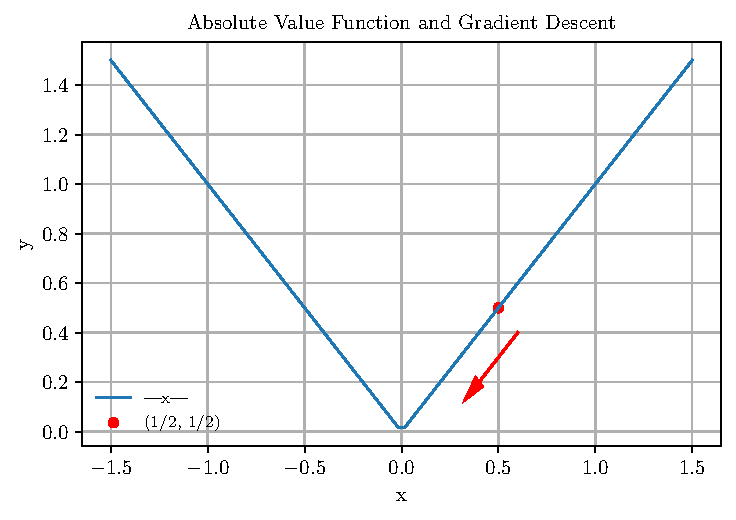
\includegraphics[width=0.7\textwidth]{plots/abs_val_func.pdf}
    \caption{The absolute value function $|x|$ and Gradient Descent with
        $x_0 = \frac{1}{2}$ and $t_k = 1$.
        We see that the Gradient jumps from $-1$ to $1$ at $x = 0$.
    }
    \label{fig:abs_value_function}
\end{figure}

With \emph{any constant step size} $t_k$,
Gradient Descent will oscillate forever on this problem.
One possible solution is to \emph{decay} the step size
$t_k$ during the optimization process.
However, the nature of this decay must be carefully chosen
as it can lead to the method getting stuck before
reaching the global minimum.

\subsection{Line Search}

A perhaps more elegant solution to the step size problem
is to simply \emph{search} for the best step size $t_k$
at every iteration.
In the example of Figure~\ref{fig:abs_value_function},
we would quickly find the global minimum at $x = 0$.

% Define exact line search, many function calls

% Armijo-Wolfe conditions (with images)

% Define inexact line search as "algorithm" block
% Explain why it works on non-smooth functions

% We now expand on the line search approaches for non-smooth optimization

% Explain that exact line search tries to find the global minimizer of f in the
% given search direction, potentially requiring many function evaluations
In an \emph{exact line search}, we attempt to solve the one-dimensional
subproblem
\begin{equation}
    t_k = \underset{t > 0}{\arg\min} \; f\bigl(x_k + t\, p_k\bigr),
\end{equation}
which can cost many function evaluations.
In Gradient Descent, an exact line search results in the
next gradient being orthogonal to the current gradient.
Often, this method quickly approaches the global minimum
taking very large steps initially, but can end up
taking many small
`zig-zag' steps once the method is near the minimum.

% TODO: FINISH FROM HERE
\subsection{Armijo-Wolfe Conditions}
% Introduce the concept of "sufficient decrease" (Armijo) and "curvature"
% (Wolfe) as a more efficient alternative
Instead of searching for exactly the best step size, a `good enough'
step size may suffice as the search direction likely changes in
the next step anyways.

\begin{align}
    f\bigl(x_k + t_k\,p_k\bigr)              & \le f(x_k)
    + c_1\, t_k \,\nabla f(x_k)^T p_k, \tag{Armijo}                                       \\[6pt]
    \nabla f\bigl(x_k + t_k\,p_k\bigr)^T p_k & \ge c_2 \,\nabla f(x_k)^T p_k. \tag{Wolfe}
\end{align}

\subsection{Inexact Line Search Algorithm}
% Present a simple pseudo-code for inexact line search using Armijo-Wolfe
\begin{algorithm}[H]
    \caption{Inexact Line Search (Armijo-Wolfe)}
    \SetAlgoLined \KwIn{Current point $x_k$, direction $p_k$, constants $0< c_1
            < c_2 < 1$, initial step $\alpha_{\text{max}}>0$.} \KwOut{Step size $t_k >
            0$.} Set $t \gets \alpha_{\text{max}}$ \; \While{Armijo or Wolfe condition
        is not satisfied}{ reduce $t$ by a factor, e.g., $t \gets \beta\, t$ (for
        some $\beta < 1$)\; } \textbf{return} $t$ as $t_k$.
\end{algorithm}

\subsection{Why These Methods Work for Non-smooth Functions}
% Non-smooth "corners" cause oscillations for constant step sizes but line
% search can adapt step size to maintain progress
Line search methods adaptively adjust the step size so that gradient-based
methods avoid large oscillations near non-differentiable \emph{corners} (such as
$|x|$ at $x=0$) and still make progress toward minimizing $f$ [1]. Precisely
because they do not rely on a fixed learning rate, they can sidestep the
pitfalls of constant-step approaches, helping the algorithm locate or
approximate subgradients more reliably and converge even when the function is
not strictly differentiable at certain points.


\end{document}